\section{Results}
To demonstrate the potency of our approach we have solved the TSP for multiple
datasets. We compare the optimal results to the results found using the
combination of renormalization and simulated annealing. To analyze the quality
of the proposed technique the state of the system while seeking the solution
for two different datasets is compared.

The first data set which
contains 198 cities shows an ideal run of the algorithm. The second dataset
contains 575 cities and, as we shall see, is a worst case scenario for this
algorithm.

\ctable[caption={The results found compared to the shortest route for various
	cities},
		 label={fig:results},
		 figure]{c}{}{\FL
		 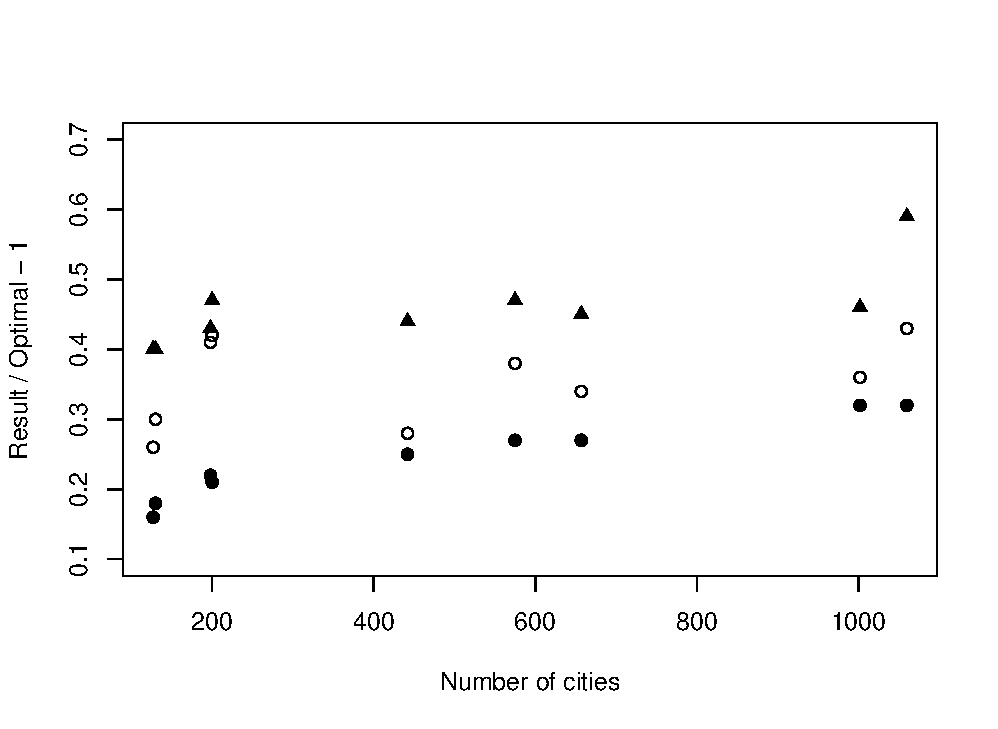
\includegraphics[width=7cm]{fig/results}
		 \LL}

\ctable[caption={The location of the cities in the 198 cities problem},
		 label={fig:d198},
		 figure]{c}{}{\FL
		 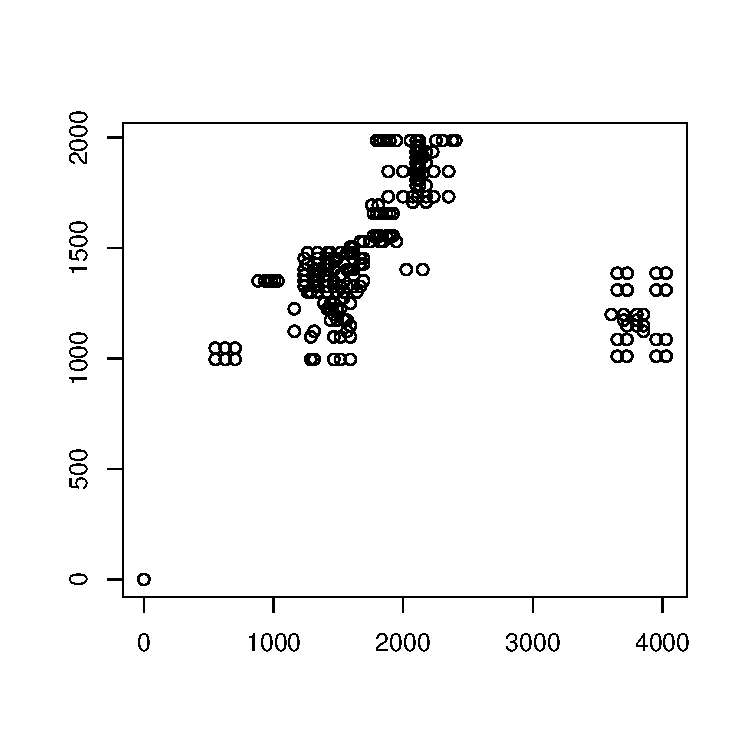
\includegraphics[width=7cm]{fig/d198cities}
		 \LL}

\ctable[caption={The location of the cities in the 575 cities problem},
		 label={fig:rat575},
		 figure]{c}{}{\FL
		 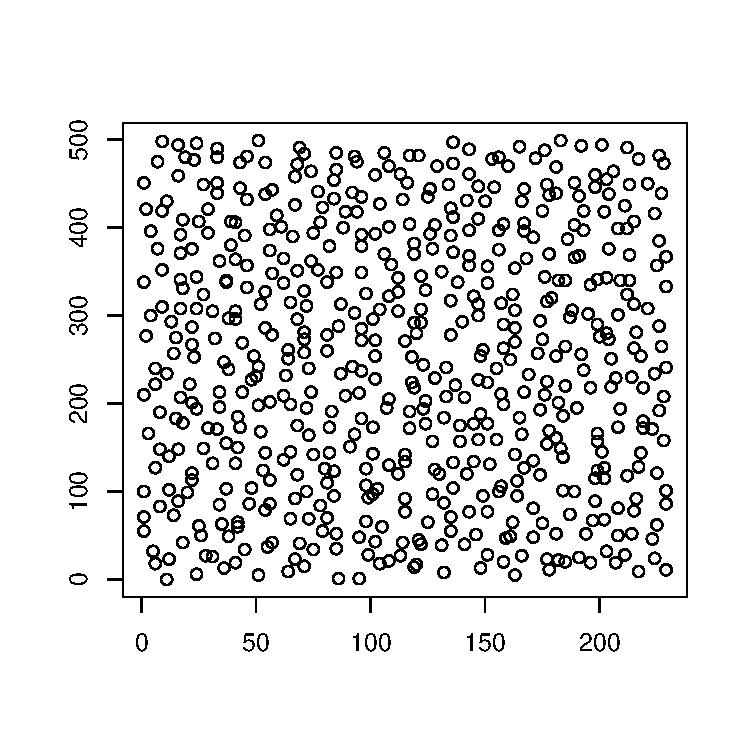
\includegraphics[width=7cm]{fig/rat575cities}
		 \LL}

\ctable[caption={Properties of the system when seeking the shortest route
		among 575 cities},
		label={fig:rat575},
		figure,
		star]{c}{}{\FL
		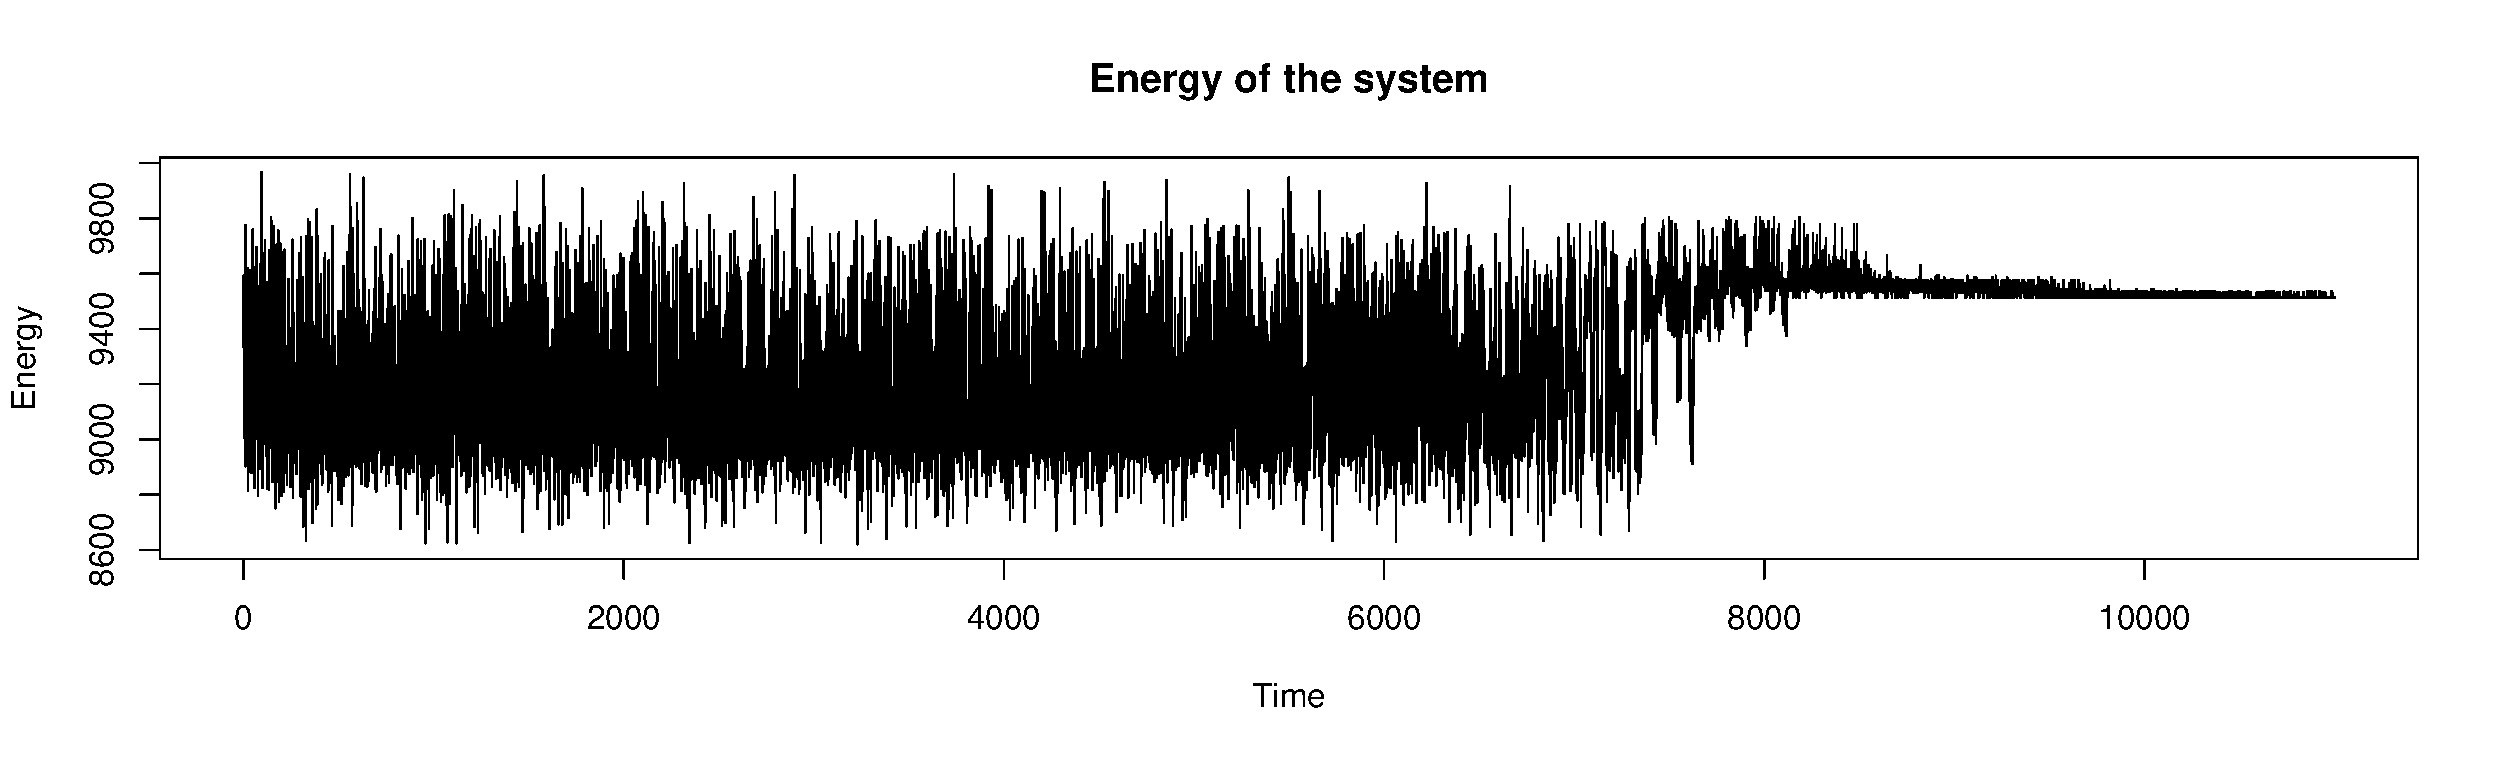
\includegraphics[width=15cm]{fig/rat575energy}\NN
		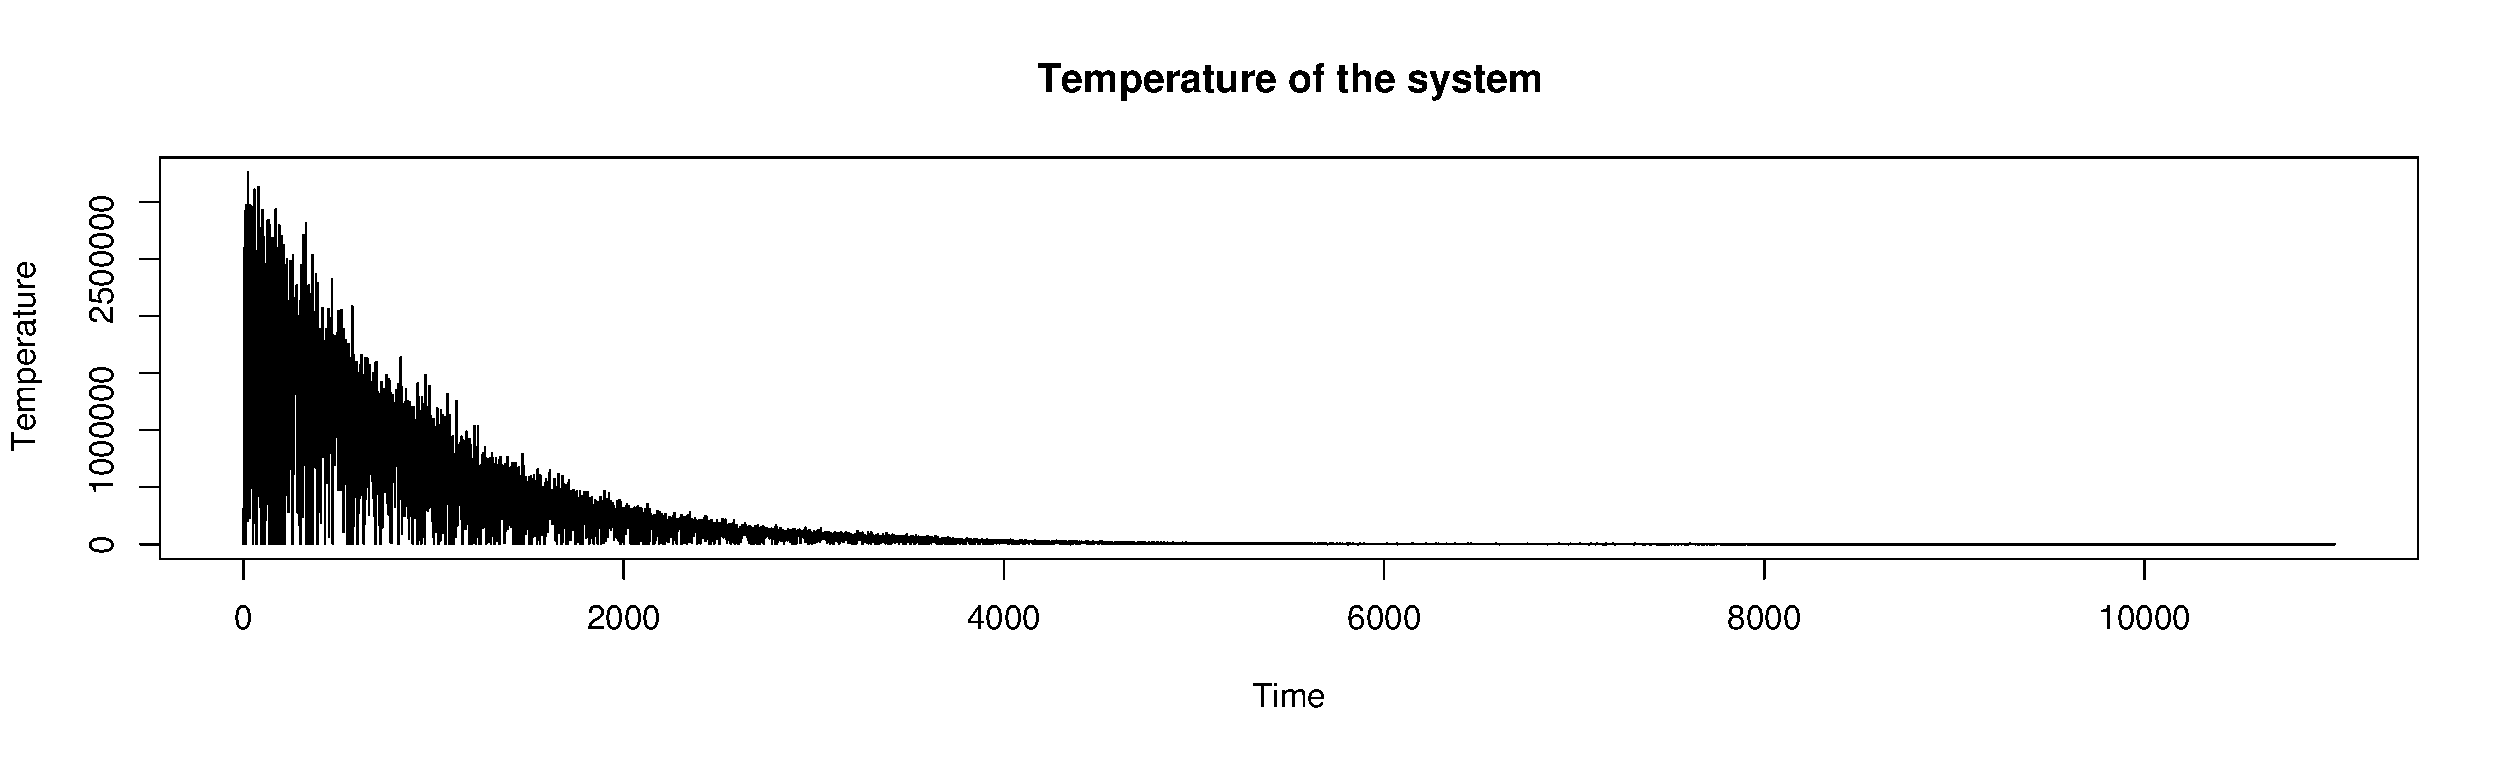
\includegraphics[width=15cm]{fig/rat575temp}\NN
		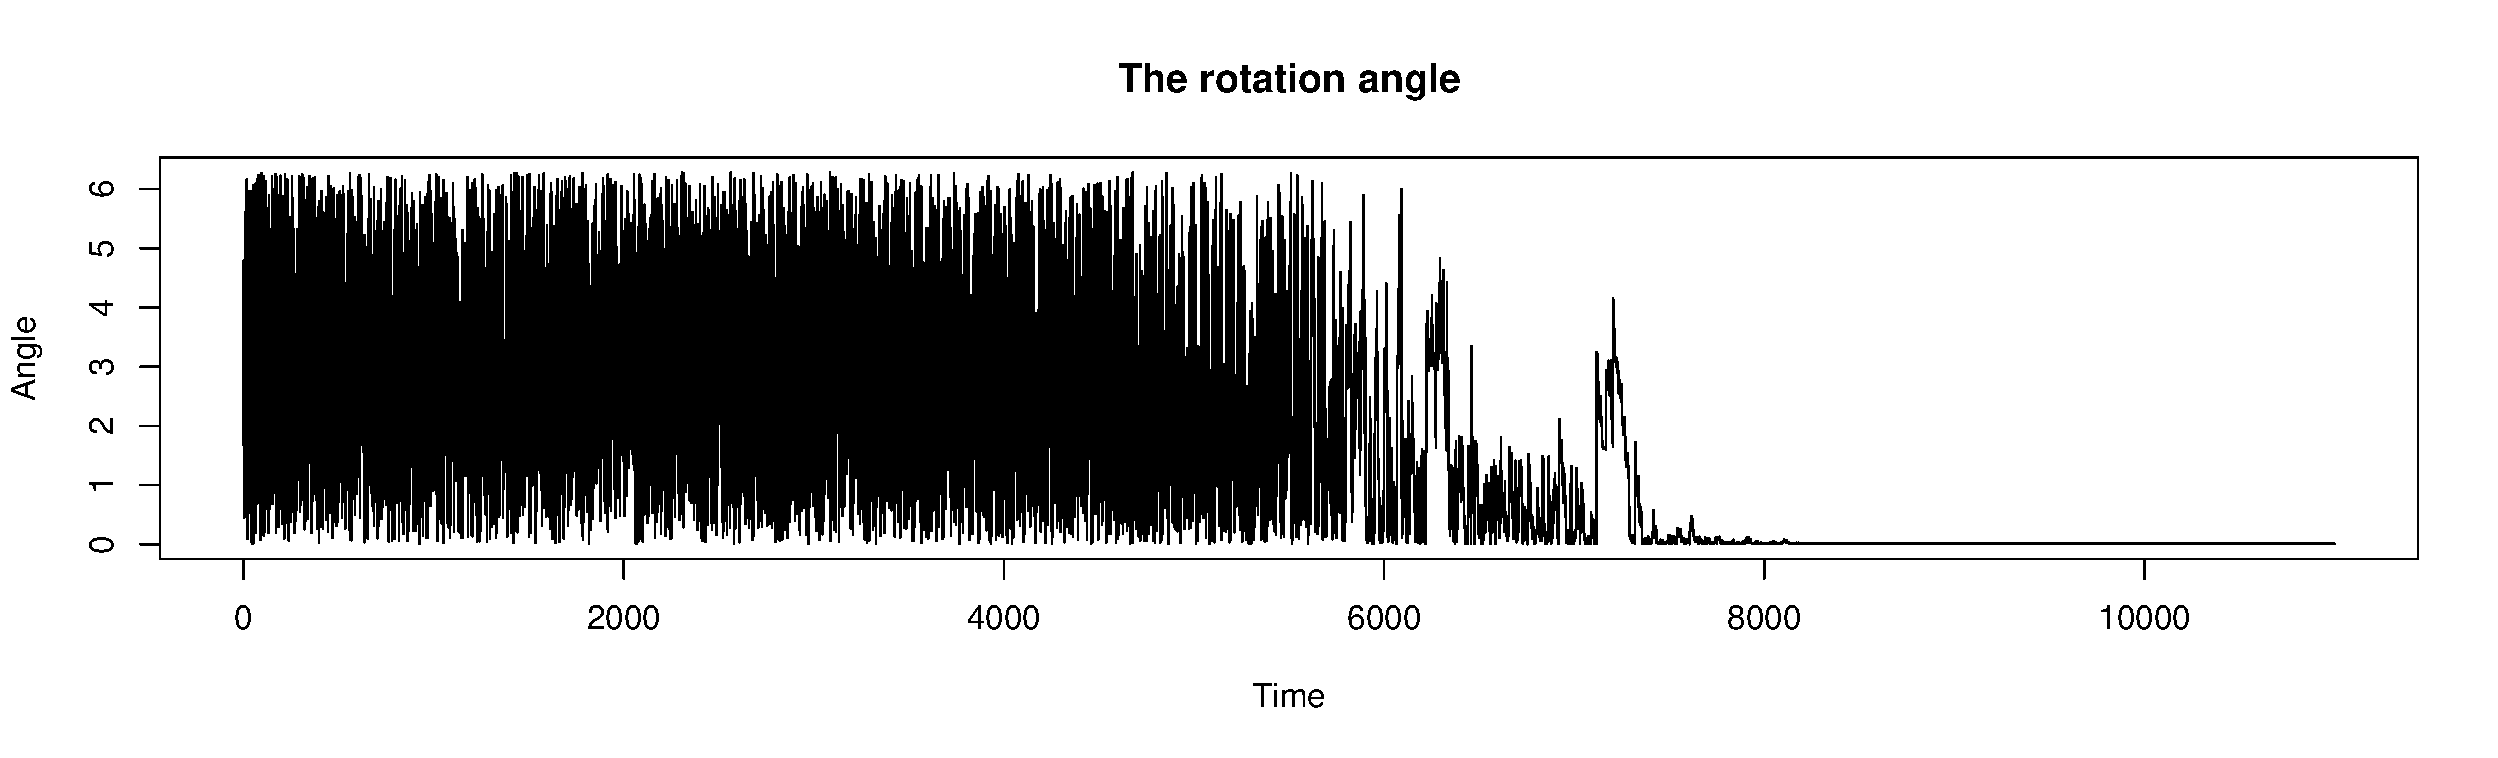
\includegraphics[width=15cm]{fig/rat575rotation}\NN
		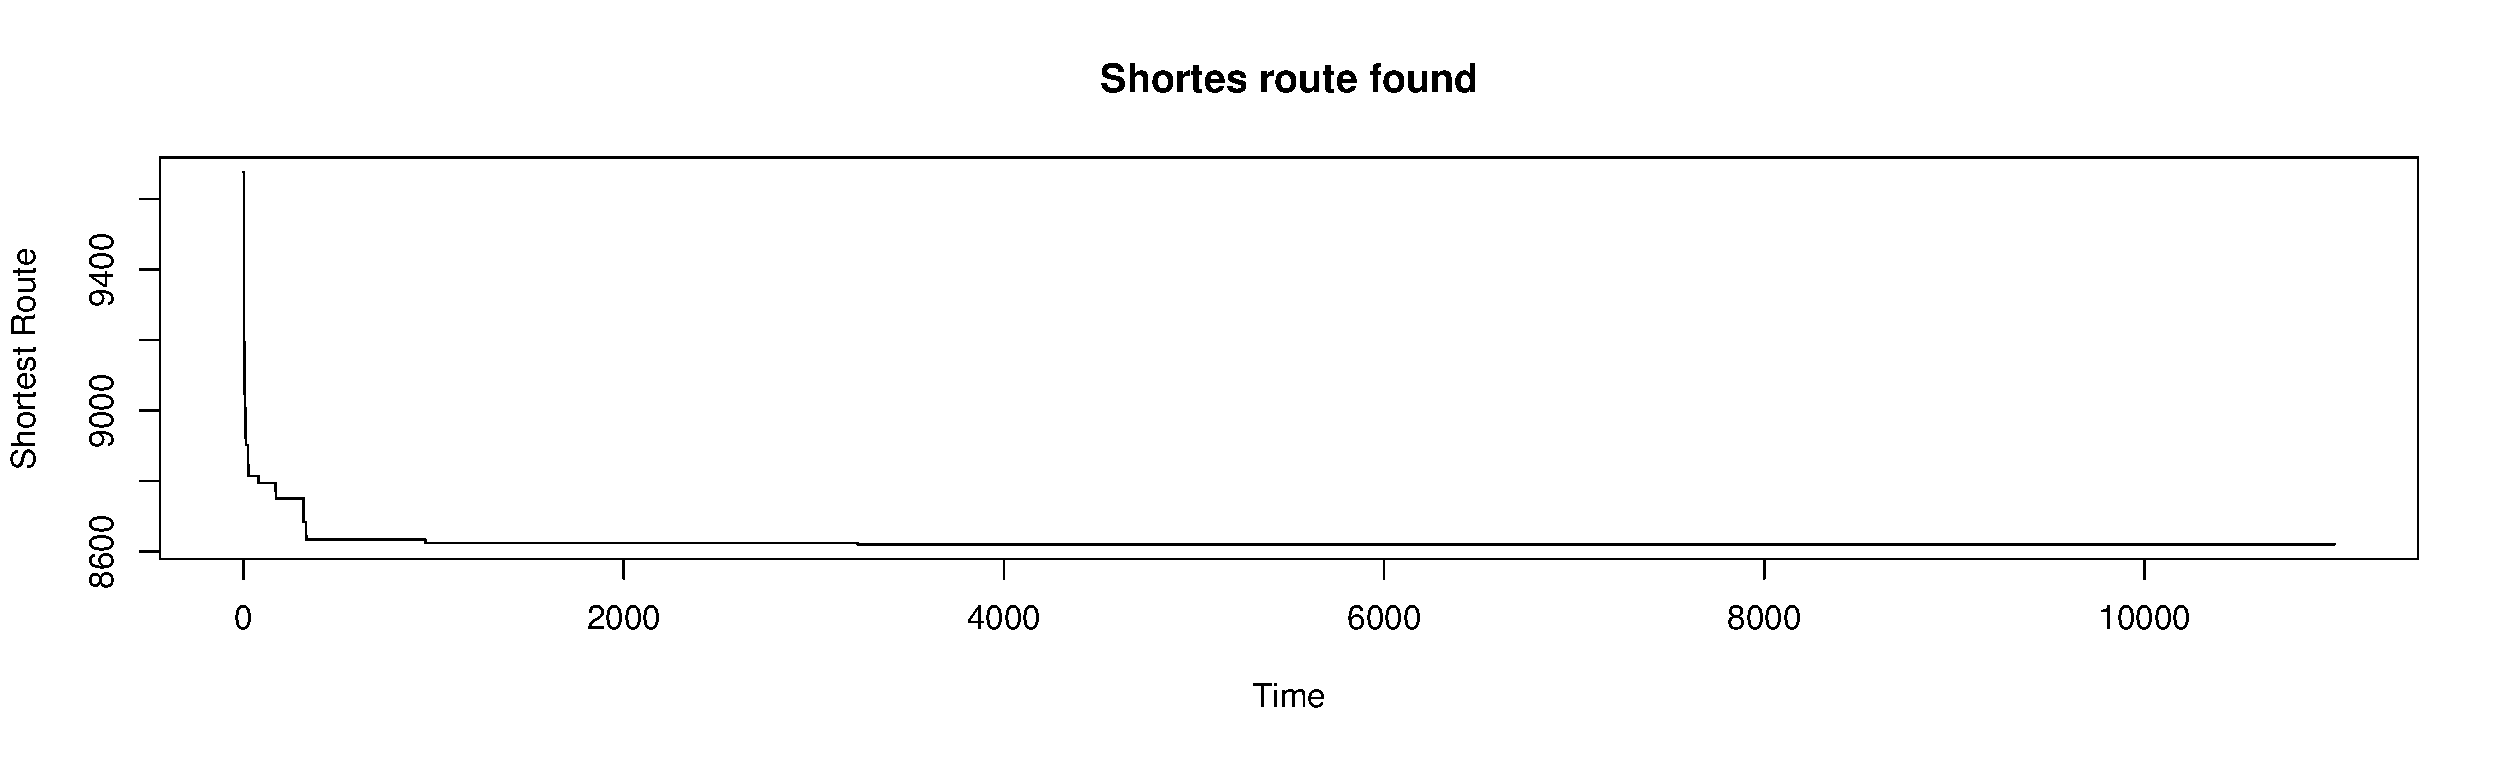
\includegraphics[width=15cm]{fig/rat575shortest}\LL}

\ctable[caption={Properties of the system when seeking the shortest route
		among 198 cities},
		label={fig:198},
		figure,
		star]{c}{}{\FL
		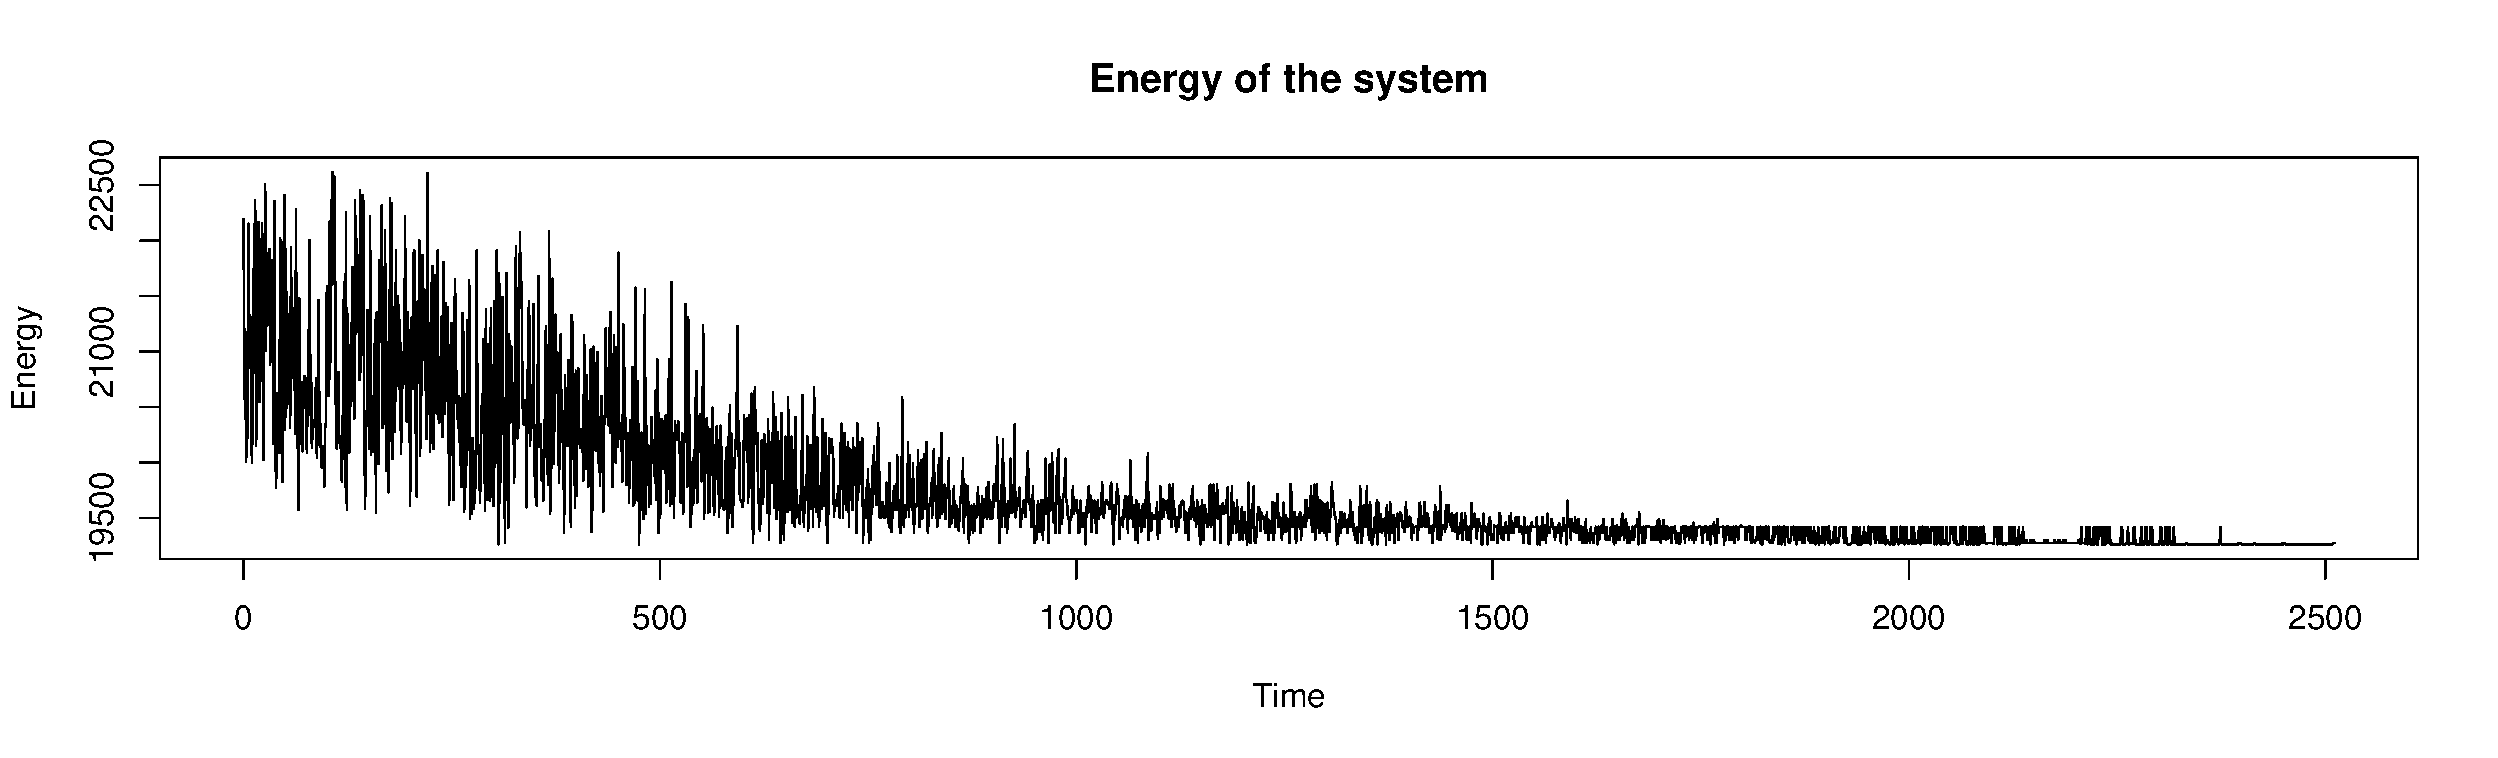
\includegraphics[width=15cm]{fig/d198energy}\NN
		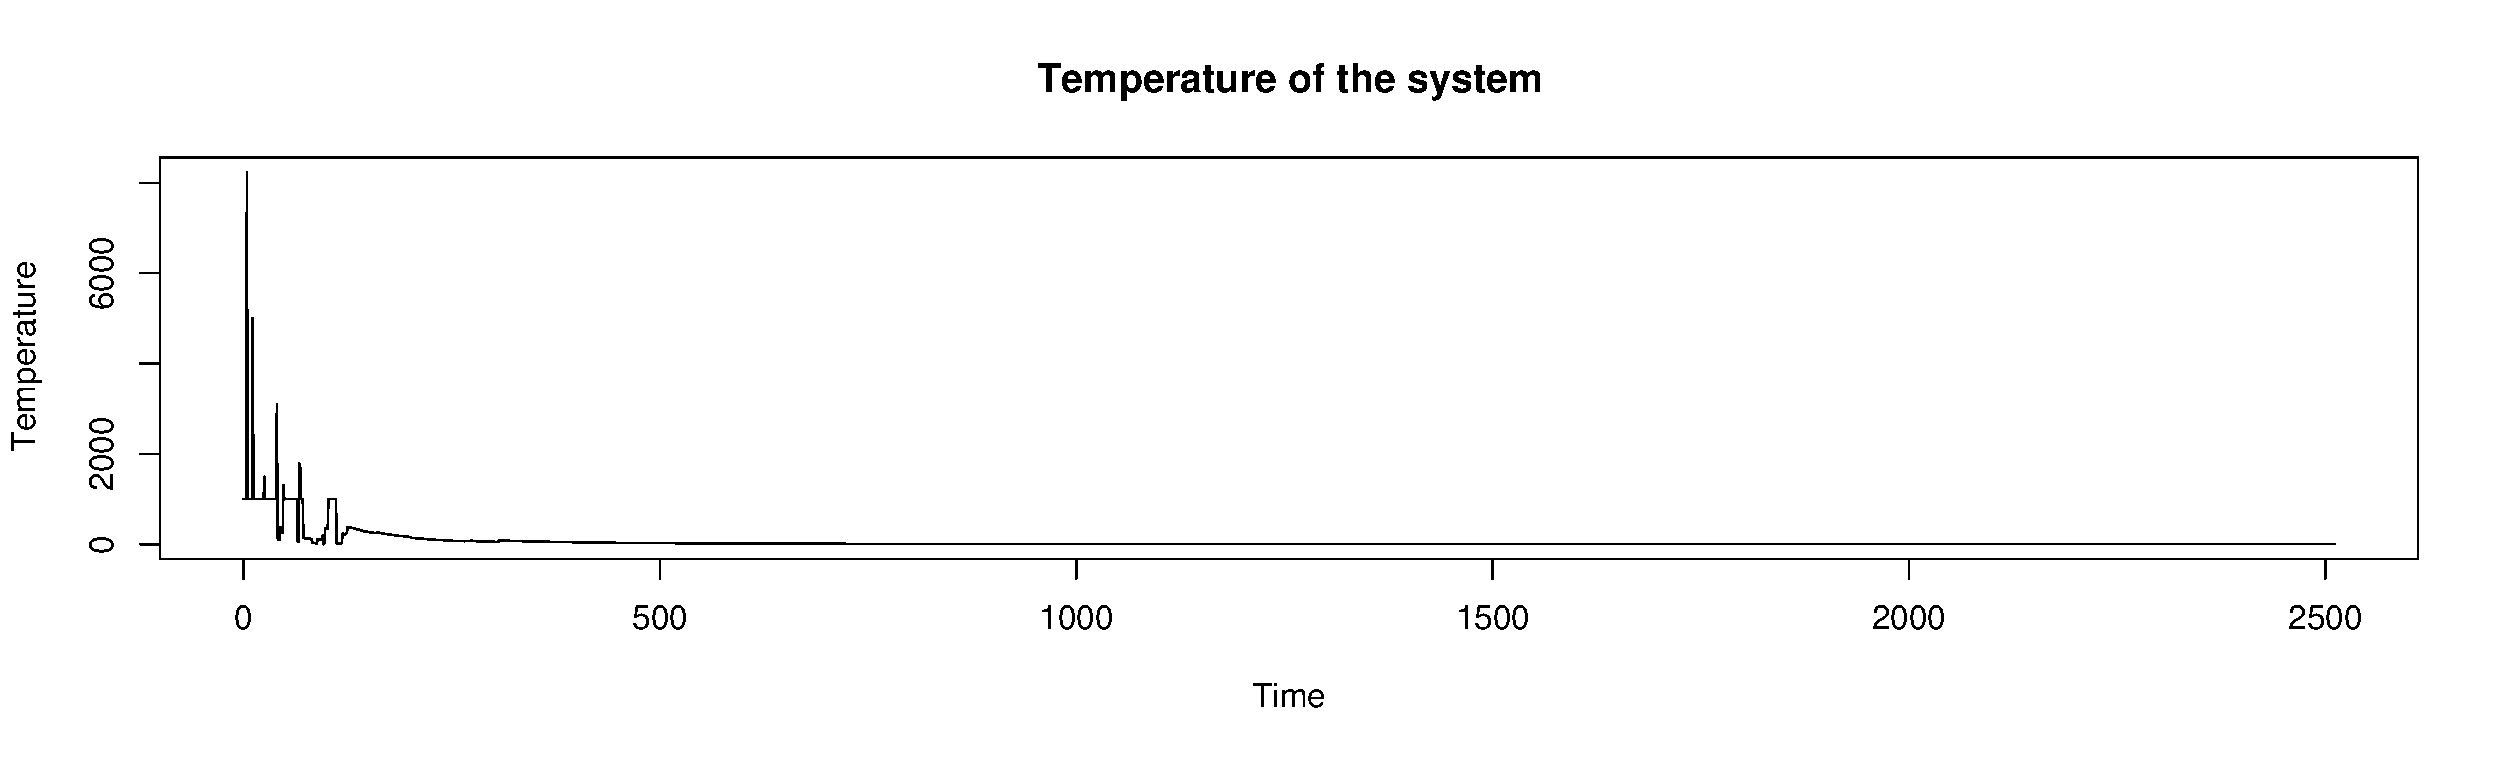
\includegraphics[width=15cm]{fig/d198temp}\NN
		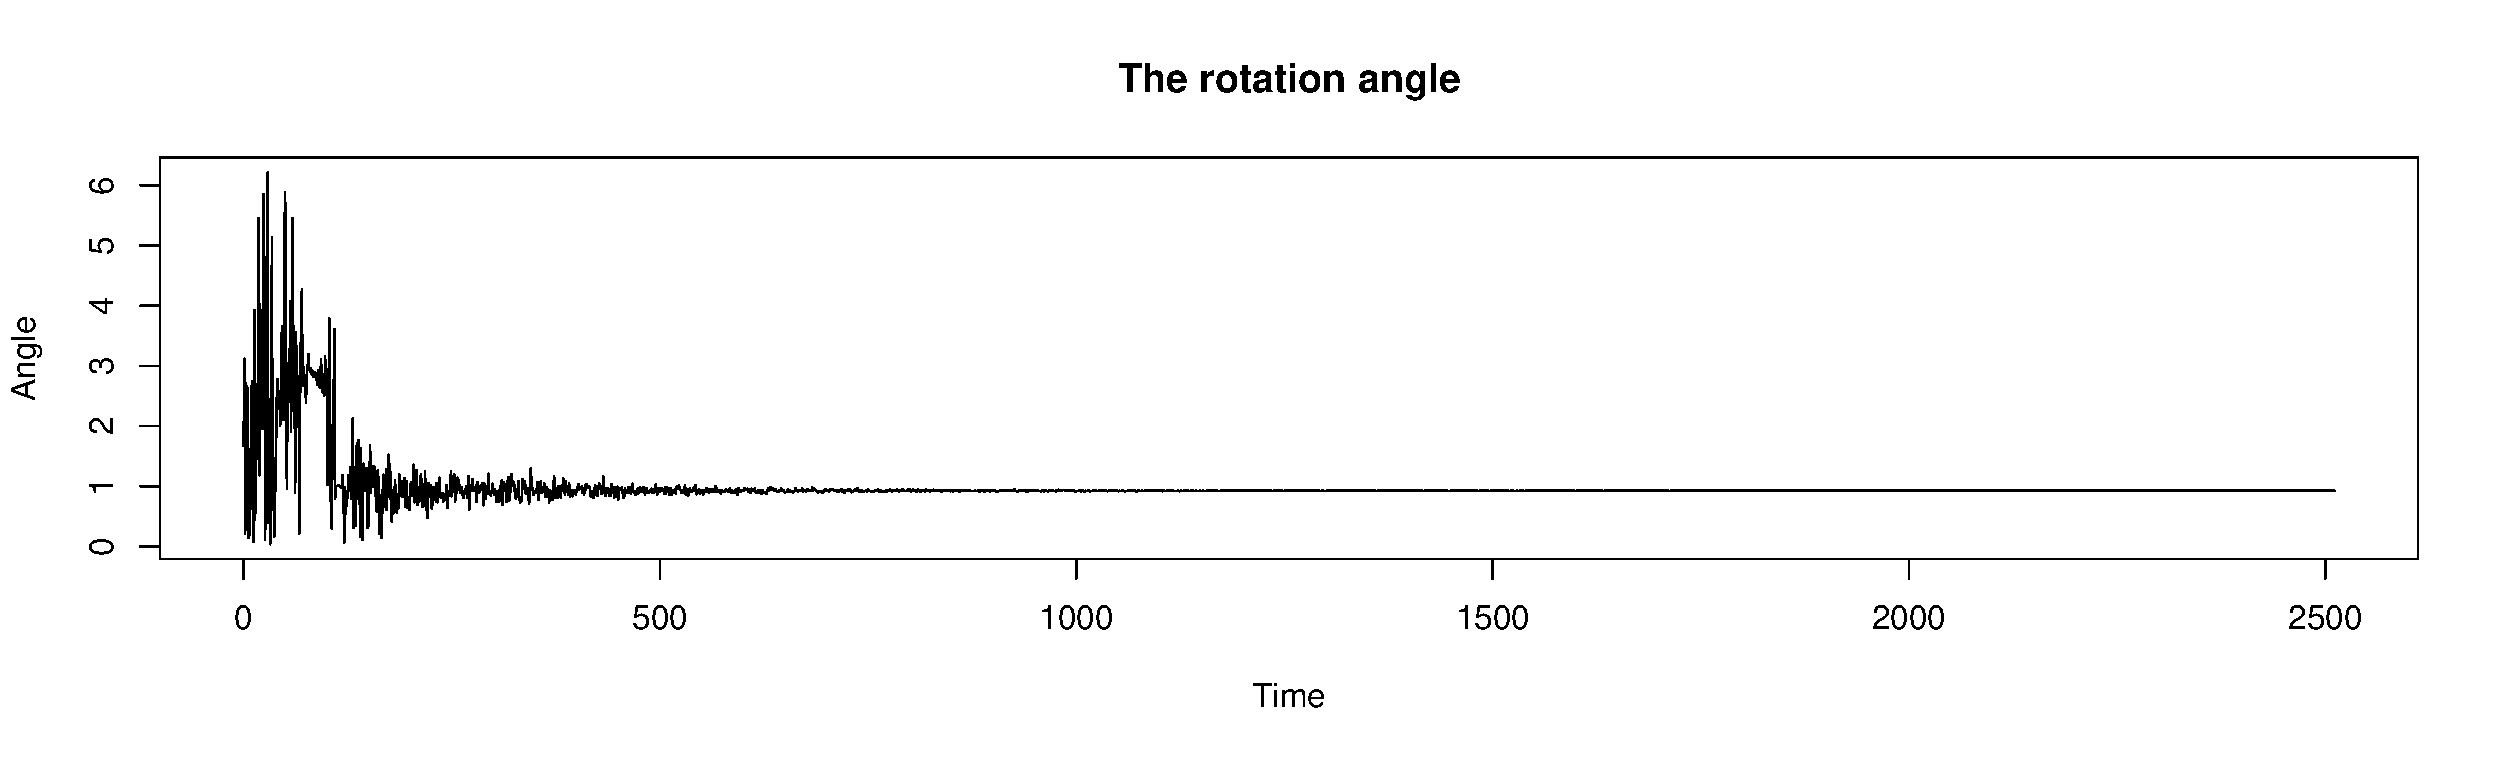
\includegraphics[width=15cm]{fig/d198rotation}\NN
		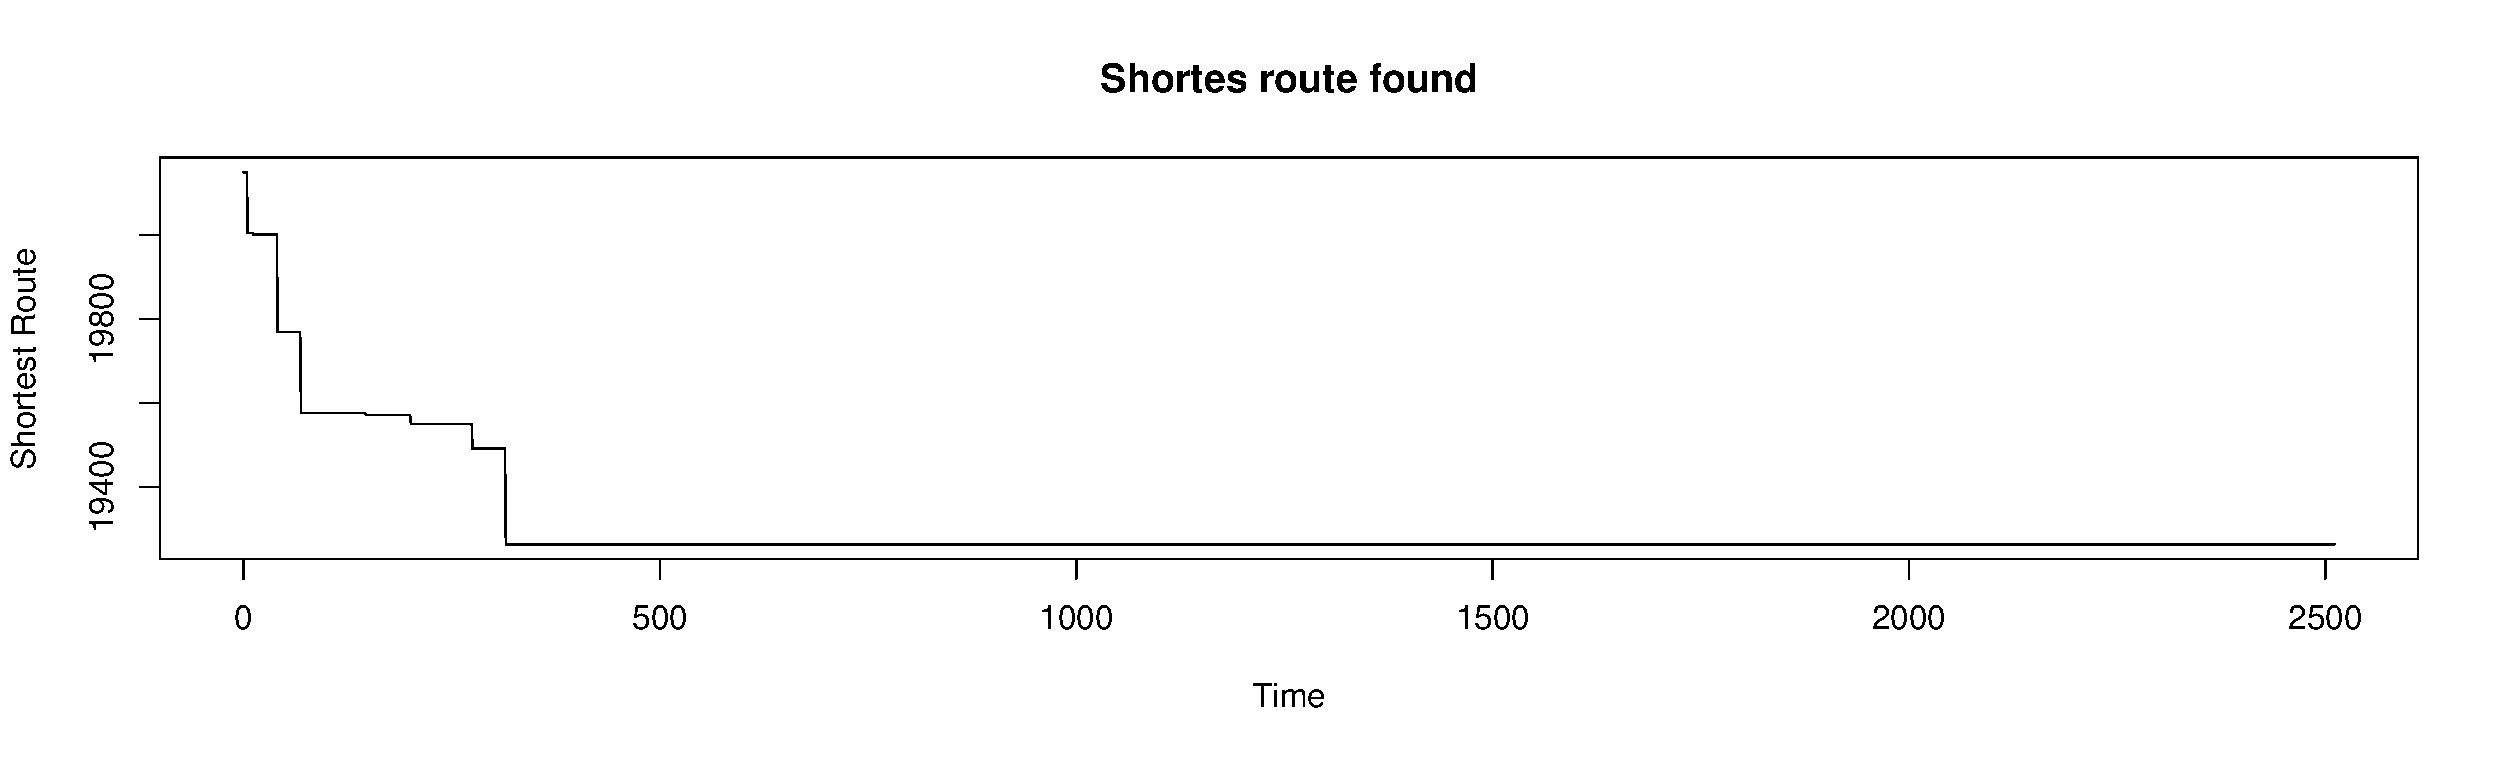
\includegraphics[width=15cm]{fig/d198shortest}\LL}


% vim:ft=tex:spell spelllang=en:autoindent

